\begin{pastexam}[label={px:df3-109-ds-05}]{地方三等資訊處理 109 年 第五題}
（申論；10 分）

請利用堆積排序法（Heap Sort）將圖2逐步建立成 Min Heap，並將數字從小到大逐一列舉。（10分）
\begin{center}
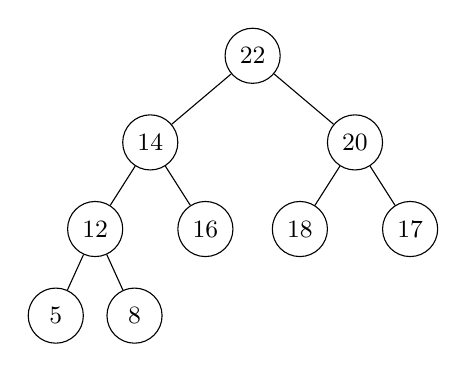
\begin{tikzpicture}[v/.style={circle,draw,minimum size=7mm,inner sep=0pt,font=\small},
    level distance=11mm, level 1/.style={sibling distance=26mm}, level 2/.style={sibling distance=14mm},
    level 3/.style={sibling distance=10mm}]
\node[v] {22}
  child {node[v] {14} child {node[v] {12} child {node[v] {5}} child {node[v] {8}}} child {node[v] {16}}}
  child {node[v] {20} child {node[v] {18}} child {node[v] {17}}};
\end{tikzpicture}\\[2pt]
圖2
\end{center}
\end{pastexam}

\begin{pastsoln}
答案：建好的 Min Heap 依層序是 $5, 8, 17, 12, 16, 18, 20, 22, 14$；由小到大列出 $5, 8, 12, 14, 16, 17, 18, 20, 22$。

圖 2 是一棵完整二元樹，依層序存成陣列 $A[1..9] = \langle 22, 14, 20, 12, 16, 18, 17, 5, 8\rangle$（$A[i]$ 的子節點是
$A[2i]$、$A[2i + 1]$）。 題目沒有說「依序插入」，照堆積排序的做法用\textbf{由下而上}建堆（資結書第~8.2~節、
虛擬碼~8.3，這裡是最小堆積的版本）：從最後一個內部節點 $\lfloor 9/2 \rfloor = 4$ 倒著做到 $1$，每次把 $A[i]$
往下沉：和較小的子節點比，較小的子節點比它小就交換，一路沉到不能再沉。

\textbf{建堆}：
\begin{center}
\small
\begin{tabular}{cp{0.42\linewidth}l}
\toprule
$i$ & 下沉過程 & 之後的陣列 \\
\midrule
 & & $22, 14, 20, 12, 16, 18, 17, 5, 8$ \\
4 & 12 的子節點 5、8，和 5 交換 & $22, 14, 20, 5, 16, 18, 17, 12, 8$ \\
3 & 20 的子節點 18、17，和 17 交換 & $22, 14, 17, 5, 16, 18, 20, 12, 8$ \\
2 & 14 和子節點 5 交換；到位置 4，再和子節點 8（12、8 中較小）交換 & $22, 5, 17, 8, 16, 18, 20, 12, 14$ \\
1 & 22 和 5 交換；到位置 2 和 8 交換；到位置 4 和 12 交換 & $5, 8, 17, 12, 16, 18, 20, 22, 14$ \\
\bottomrule
\end{tabular}
\end{center}
建好的 Min Heap：
\begin{center}
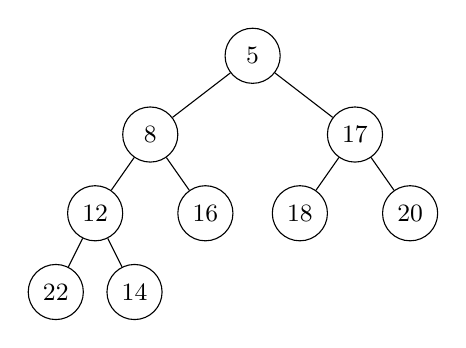
\begin{tikzpicture}[v/.style={circle,draw,minimum size=7mm,inner sep=0pt,font=\small},
    level distance=10mm, level 1/.style={sibling distance=26mm}, level 2/.style={sibling distance=14mm},
    level 3/.style={sibling distance=10mm}]
\node[v] {5}
  child {node[v] {8} child {node[v] {12} child {node[v] {22}} child {node[v] {14}}} child {node[v] {16}}}
  child {node[v] {17} child {node[v] {18}} child {node[v] {20}}};
\end{tikzpicture}
\end{center}
檢查：每個父節點都不大於子節點（$5 \le 8, 17$；$8 \le 12, 16$；$17 \le 18, 20$；$12 \le 22, 14$）。

\textbf{逐一取出}：每次取出堆頂（目前最小值），把最後一個元素移到堆頂、堆積大小減一，再從堆頂往下沉。
\begin{center}
\small
\begin{tabular}{cp{0.42\linewidth}l}
\toprule
取出 & 最後一個移到堆頂後下沉 & 剩下的堆積 \\
\midrule
5 & 14 上來，和 8、12 交換 & $8, 12, 17, 14, 16, 18, 20, 22$ \\
8 & 22 上來，和 12、14 交換 & $12, 14, 17, 22, 16, 18, 20$ \\
12 & 20 上來，和 14、16 交換 & $14, 16, 17, 22, 20, 18$ \\
14 & 18 上來，和 16 交換（位置 2 的子節點 22、20 都比 18 大） & $16, 18, 17, 22, 20$ \\
16 & 20 上來，和 17 交換 & $17, 18, 20, 22$ \\
17 & 22 上來，和 18 交換 & $18, 22, 20$ \\
18 & 20 上來，子節點 22 比它大，不動 & $20, 22$ \\
20 & 22 上來 & $22$ \\
22 & & 空 \\
\bottomrule
\end{tabular}
\end{center}
取出的順序就是由小到大：$\mathbf{5, 8, 12, 14, 16, 17, 18, 20, 22}$。 （在原陣列上做堆積排序時，取出的堆頂放到
陣列尾端，用 Min Heap 會得到由大到小的陣列；題目要的是「逐一列舉」，就是上面取出的順序。）

若改用「依序插入」建堆（把 22, 14, 20, 12, 16, 18, 17, 5, 8 一個一個插入空的 Min Heap，每次往上浮），得到的
是 $5, 8, 17, 12, 16, 20, 18, 22, 14$，和由下而上建出來的不同（18、20 的位置對調），但一樣是合法的 Min Heap，
取出的順序也相同。
\end{pastsoln}
